%
%

\begin{titlepage}
\begin{center}
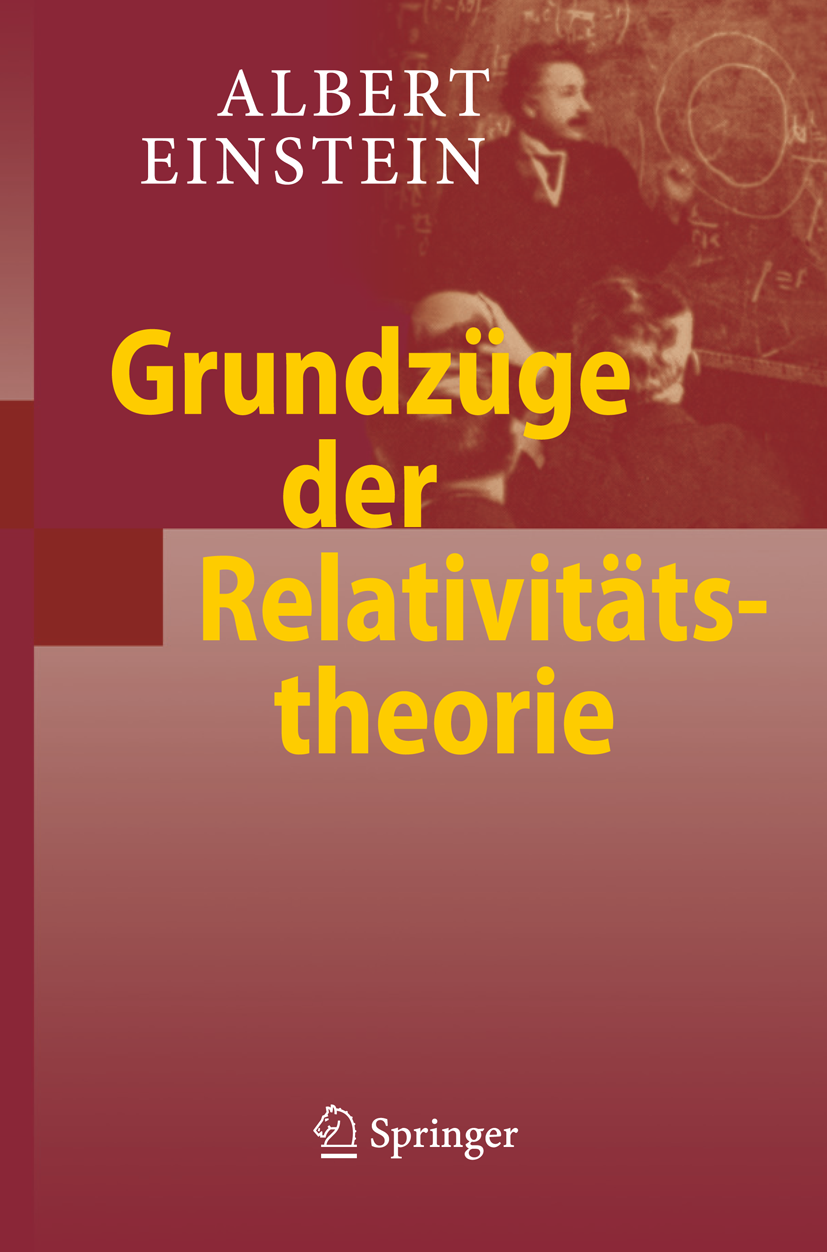
\includegraphics[]{./img/9783540878469.png}
\end{center}
\end{titlepage}

%CREATE HERE A TITLE PAGE AS YOU LIKE. My proposal is:
%%%Moja Strona Tytulowa (do wyboru)
\newcommand{\HRule}{\rule{\linewidth}{0.5mm}}
\begin{titlepage}
\begin{center}

\HRule \\[0.3cm]
% author
% https://tex.stackexchange.com/questions/8351/what-do-makeatletter-and-makeatother-do
\makeatletter
\textsc{\Large \@author} \\[0.3cm]

\includegraphics[width=8.5cm]{img/coverimg.jpg} \\[0.3cm]
% title
{ \Huge \bfseries \@title} \\%[0.1cm]
\makeatother
\HRule \\[0.3cm]

% Optionally translator and publishing house
% The Translator
\begin{minipage}{0.4\textwidth}
\begin{flushleft} \small
\emph{Translated by:}\\
Good Translator %here the translator
\end{flushleft}
\end{minipage}
% Publishing House
\begin{minipage}{0.4\textwidth}
\begin{flushright} \small
\emph{Published by:} \\
\textsc{Springer} % here the publishing house
\end{flushright}
\end{minipage}

\end{center}
\end{titlepage}



%%%SIMPLE TITLEPAGE
%\maketitle %thispagestyle{empty}
%\clearpage
%\setcounter{tocdepth}{6}


%TUTAJ PISZ ALBO ZROB \INCLUDE{} LUB \INPUT{}


%%%%%%%%%%%%%%%%
\subsection*{Vorwort zur 1.\ Auflage der \enquote{Vier Vorlesungen über Relativitätstheorie}}
%\label{sec:vor-1}
%%%%%%%%%%%%%%%%

In der vorliegenden Ausarbeitung von vier Vorträgen, die ich an der Universität Princeton im Mai 1921 gehalten habe, wollte ich die Hauptgedanken und mathematische Methoden der Relativitätstheorie zusammenfassen. Dabei habe ich mich bemüht, alles weniger Wesentliche wegzulassen, das Grundsätzliche aber doch so zu behandeln, daß das Ganze als Einführung für alle diejenigen dienen kann, welche die Elemente der höheren Mathematik beherrschen, aber nicht allzuviel Zeit und Mühe auf den Gegenstand verwenden wollen. Auf Vollständigkeit kann diese kurze Darlegung selbstverständlich keinen Anspruch machen, zumal ich die feineren, mehr mathematisch interessanten Entwicklungen, welche sich auf Variationsrechnung gründen, nicht behandelt habe. Mein Hauptziel war es, das Grundsätzliche in dem ganzen Gedankengang der Theorie klar hervortreten zu lassen.

Januar 1922 \hfill A.\ \textsc{Einstein} \hspace{1.5em}
